\documentclass[conference]{IEEEtran}
\IEEEoverridecommandlockouts
% The preceding line is only needed to identify funding in the first footnote. If that is unneeded, please comment it out.
\usepackage{cite}
\usepackage{amsmath,amssymb,amsfonts}
\usepackage[nottoc]{tocbibind}
\usepackage{algorithmic}
\usepackage{gensymb}
\usepackage{graphicx}
\usepackage{textcomp}
\usepackage{xcolor}
\usepackage{subfig}

\newcommand{\ra}[1]{\renewcommand{\arraystretch}{#1}}

%bibliography file "bibliography.bib"

\def\BibTeX{{\rm B\kern-.05em{\sc i\kern-.025em b}\kern-.08em
    T\kern-.1667em\lower.7ex\hbox{E}\kern-.125emX}}
\begin{document}
\title{Comparing the Performance of 3D Classification Models on Various Datasets\\}

\author{\IEEEauthorblockN{Kyle Lukaszek}
\IEEEauthorblockA{\textit{School of Computer Science} \\
\textit{University of Guelph}\\
Guelph, Canada \\
klukasze@uoguelph.ca}
\and
\IEEEauthorblockN{Luke Janik-Jones}
\IEEEauthorblockA{\textit{School of Computer Science} \\
\textit{University of Guelph}\\
Guelph, Canada \\
ljanikjo@uoguelph.ca}
}

\maketitle

% --------------  ABSTRACT  -----------------

\begin{abstract}
This paper presents a comparative analysis of various 3D classification models across several popular datasets, evaluating existing models against our novel model derived from researched models. The existing models we compare include VoxNet \cite{7353481}, and a novel approach by JunYoung Gwak that we reference as 3DCNN \cite{gwak20153d}. Additionally, a Python framework is introduced, facilitating the generation of voxelized 3D objects from different datasets in a compressed, potentially mobile-friendly format. Popular datasets—ModelNet40 \cite{7298801}, ShapeNet/PartNet \cite{shapenet2015}\cite{qi2017pointnetplusplus}, and Toys4K \cite{stojanov2021using}—are used to evaluate model performance and their ability to classify specific object types. Findings offer insights into each model's capabilities, and their suitability for specific research domains, as well as insights into the practicality of the tested datasets.
\end{abstract}

% --------------  INTRODUCTION  -----------------

\section{Introduction}

Over the years, the field of machine learning has evolved rapidly, continually pushing the boundaries of what is achievable with artificial intelligence. In this ever-changing field, 3D object classification stands out as a particularly difficult challenge. Conceptually, it would be simple to extend a two-dimensional approach to the third dimension, but in reality, many over the years have found that it is difficult to determine what methods yield higher performance\cite{7353481}. In the interest of determining what makes a strong model, this paper compares three different convolutional neural networks. Each one takes the same input, yet by analyzing their performance over several datasets we can observe how their differences affect their handling of varied data. As one of these models is entirely our own, we are also able to observe the evolution of machine learning as we analyze it in comparison to models that were constructed not even ten years prior.

Furthermore, our study delves into the evaluation of these models using industry-standard datasets including ModelNet40, ShapeNetPart, and Toys4K. This ensures that the outcomes offer insights into each model's capabilities and ability to classify distinct object categories. Notably, our findings delineate model efficacy, shedding light on their suitability for various research applications. The meticulous comparison across various measures and datasets not only reveals the strengths and weaknesses of each CNN but can also serve as a valuable benchmark for future developments in 3D object classification.

The juxtaposition of a mobile-friendly 3D object classifier and a voxel-based object reconstruction algorithm\cite{math9182288} presents compelling prospects for subsequent projects. Fig \ref{fig:plane} shows a voxelized transformation of an airplane. This paper not only compares model performance but also underscores their relevance in varied research applications, contributing pivotal insights to the evolving field of 3D classification. As the demand for intelligent systems capable of understanding and interpreting three-dimensional environments continues to rise, our research plays a crucial role in guiding the design and implementation of effective 3D object classifiers, opening new avenues for innovation in machine learning.

\begin{figure}
    \centering
    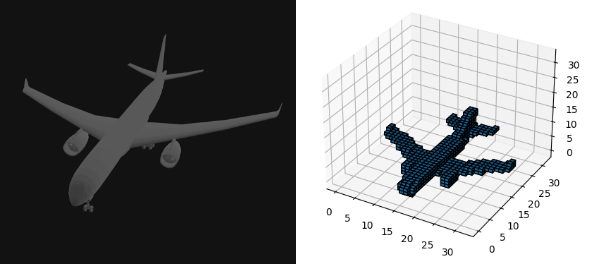
\includegraphics[scale=0.5]{Images/airplane 3D.png}
    \caption{32x32x32 Voxelized 3D Object}
    \label{fig:plane}
\end{figure}

\section{Motivation and Objectives}

The main objective of this project is to compare the strengths and overall performance of various 3D classification models over several datasets. In the past few years, object classification algorithms have grown significantly more powerful, and our goal is to observe this growth through the comparison of these models. Initially, we wished to compare and contrast several of these algorithms over three different datasets. Since then, we've had to scale back our scope to just three models, tested over those three datasets. These models are VoxNet, a 3DCNN, and a CNN of our design. Each of these neural networks interprets a voxel grid to classify an object into one of several categories based on which of the three datasets is input. With these three models, we can compare their accuracy, F-measure, and Mean Squared Error to determine which is the greatest performing of the three.

Another main objective of ours is for the neural net we designed to have performance comparable to either of the two other models that we implemented. Both of these models were created in 2015\cite{gwak20153d}\cite{7353481}, and many improvements to both computer processing power as a whole and the field of machine learning have been made in the years since. With that in mind, it is possible that our model could return results equal to or surpassing either of the models we are comparing it with. The datasets that we are testing these models on are ModelNet40, ShapeNet, and Toys4K. These datasets are all robust, and each varies in the number of total objects and classes. Due to these differences, we can test the models under a variety of circumstances that give us an idea of the strengths and weaknesses of each. In doing so, we hope to demonstrate the progress that has been made in only eight years.

\section{Methodology}

\subsection{Datasets}
\subsubsection{ModelNet40}
We decided to work with ModelNet40 \cite{7298801} as our primary dataset since it provides a large number of 3D objects with a wide variety of classes and samples per class. ModelNet40 is one of the largest publicly available CAD datasets and is used as a staple benchmark for 3D object classification as it has been around since 2015. The dataset contains 12,311 CAD models from 40 categories, with 9,843 models for training and 2,468 models for testing. The dataset is pre-split into training and testing sets with a ratio of 80:20. The models are provided in .off format and are centered and normalized which makes them easy to work with. 
\subsubsection{ShapeNetPartAnnotation}
We originally chose to work with ShapeNet \cite{shapenet2015} as it is another large dataset with a wide variety of classes and samples per class. Unfortunately, ShapeNet was too large to use for training and testing on our local machines so we decided to settle for a subset of ShapeNet put together for PointNet++\cite{qi2017pointnetplusplus}. The subset we used is provided by Stanford University and contains 16,881 CAD models from 16 categories. The files provided are in .xyzn point cloud format so we had to cross-reference the files between the subset and the original ShapeNet dataset to get the .obj files. We then split the dataset into training and testing sets with a ratio of 80:20. The models are not centered, normalized, or rotated properly, so we had to do that ourselves.
\subsubsection{Toys4K}
Toys4K \cite{stojanov2021using} is a more recent dataset that was released in 2021. It contains 4,000 CAD models from 105 categories. This provides us with the largest variety of classes to work with but with the smallest number of samples per class. The files are provided in .obj format and are not centered, normalized, or rotated properly, so we had to do that ourselves. No training and testing sets are provided so we had to split the dataset ourselves with a ratio of 80:20.

\subsection{Tools and Libraries}
\subsubsection{Python}
We use Python as our primary programming language for this project. Python is a high-level, general-purpose programming language that is widely used in the field of machine learning. Python is also the language that the majority of the libraries we use are written in.

\subsubsection{PyTorch}
PyTorch \cite{paszke2017automatic} is an open-source machine learning library based on the Torch library, used for applications such as computer vision and natural language processing. We use PyTorch to build our models and to train them on the various datasets.

\subsubsection{NumPy}
NumPy \cite{harris2020array} is a Python library that we use for data preprocessing, manipulation, and compression. NumPy is a fundamental package for scientific computing in Python and is used for working with arrays and matrices. We use NumPy to store the array representations of the voxelized 3D objects and to compress them into .npz files.

\subsubsection{SciKit-Learn}
SciKit-Learn \cite{scikit-learn} is a Python library that we use to calculate our models' evaluation metrics. We use SciKit-Learn to quickly calculate the F1-Score, Mean-Squared Error, and Confusion Matrix of our models.

\subsubsection{Matplotlib}
Matplotlib \cite{Hunter:2007} is a Python library that we use for data visualization. Any graphs or plots that we generate are done using Matplotlib.

\subsubsection{CUDA Voxelizer}
CUDA Voxelizer \cite{math9182288} is a program that we use to convert 3D objects into voxelized representations. We use CUDA Voxelizer to convert .obj and .off files into .binvox files so that they can be efficiently processed in Python.

\subsubsection{Binvox}
Binvox {binvox} is a program that converts 3D objects into voxelized representations. We use Binvox as a backup voxelizer in case the CUDA Voxelizer fails to convert a 3D object into a .binvox file. Binvox is also the origin of the .binvox file format which is worth mentioning.

\subsubsection {Trimesh4}
Trimesh4 \cite{trimesh} is a Python library for loading and using triangular meshes with an emphasis on watertight surfaces. We use Trimesh4 to load the .binvox files and convert them into NumPy arrays.

\subsection{Data Preprocessing}
The nature of this project is quite demanding from a resources perspective so we had to be very careful with how we handled the data. We had to make sure we were not loading too much data into memory at once and that we were not wasting any space when storing the data. We also had to make sure that the data was in the correct format for our models to process.

\subsubsection{ShapeNetPartAnnotation}
Since we are working with a subset of ShapeNet, we had to cross-reference the files between the subset and the original ShapeNet dataset. We decided to use the ShapeNetPartAnnotation dataset from the PointNet++ paper to do this. The ShapeNetPartAnnotation dataset has the same directory structure but the files are in point-cloud format. Since the names of the files match those in the ShapeNet dataset, we just had to write a script to transfer the .obj files from ShapeNet to ShapeNetPartAnnotation.

\subsubsection{Training and Testing Sets}
Since we are working with two datasets that do not have pre-split training and testing sets, we had to split the datasets ourselves. We found that the metadata file provided by ModelNet40 was very useful for splitting a large directory of files into training and testing sets. We used the format of the metadata file and wrote a Python script to walk through the directory of files and assign them a training or testing label in the metadata file, along with their class label, and file path. Once these metadata files were created, we had CSV files that indexed the files in each dataset and we could use these files to load the data into our models.

\subsubsection{Voxelization}
The datasets we selected to train and test the models on are provided in .obj and .off formats. These formats are not ideal for our models to process so we had to convert them into a more efficient format. We selected the .binvox format as it is a binary format that is very efficient to store and process. We designed a Python class to handle the creation of the necessary voxel representations for any dataset. The class takes in the directory of the dataset and checks for an appropriate metadata file. Once the metadata file is loaded and the files are indexed, we pass the files to the CUDA Voxelizer program to convert them into .binvox files. If the CUDA Voxelizer fails to convert a file, we use Binvox as a backup voxelizer. Once a .binvox file is produced, it is loaded into Trimesh4 and converted into a NumPy array. If the dataset being converted is either ShapeNet or Toys4K, we use NumPy to apply rotations to the models so that they are all facing the same direction.

The NumPy array is then compressed into a .npz file and saved to disk. The .npz file contains the voxelized representation of the 3D object and its class labels. The class also has a method to load the .npz files into memory and return the voxelized representations and class labels as NumPy arrays.

We did not perform any data augmentation on the datasets such as rotating the models several times or adding noise \cite{7353481} \cite{gwak20153d} \cite{shaoxu20163d} as this would have increased the size of the datasets and made them more difficult to work with. We also did not perform any normalization on the voxelized representations as they are already normalized to binary. 

We had worked on a partitioned implementation of the voxelization process but we found that with the resolution we were using for the models, it did not matter. For future work, we would like to implement a partitioned voxelization process and storage strategy that would allow us to use higher resolutions since 48x48x48 voxel grids failed to fit into memory on our 32GB of RAM.

\subsubsection{Our CNN Architecture}
Our CNN is a simple 3D convolutional neural network that takes in a 32x32x32 voxel grid and outputs a classification. The model consists of 2 3D convolutional layers, 1 3D max-pooling layer, and 2 fully connected layers. The final layer is another fully connected layer with $n$ output nodes where $n$ equals the number of unique labels in the dataset the model is training on. Our model attempts to implement what we find most appealing from both VoxNet and 3DCNN and implement a bit of what we learned in class about CNNs to create a model that is still simple, yet effective. We aim to create a model that is more accurate than VoxNet, but less computationally expensive than 3DCNN. We also aim to create a model that is easy to implement and understand.

\subsection{Parameter Tuning}
For parameter tuning, we used a combination of manual tuning and grid search. We started with manual tuning to get a rough idea of what parameters worked best for each model. We then used grid search to fine-tune the parameters and find the optimal values. We used the F1-Score as our metric for parameter tuning as it is a good indicator of how well the model is performing. We also used the Mean-Squared Error and Confusion Matrix to get a better idea of how the model is performing. The only difference between the parameter tuning processes is that some datasets required more epochs than others, specifically Toys4K. We will explain why we think this happened in the Results section.

\subsection{Model Training}
Every model we implemented was trained using a very similar process. We select the dataset we want to train on and load the .npz files into memory. We call the dataloader functions we wrote to generate dataloaders from the contents of our .npz files and create our training and testing dataloaders. We use the Stochastic Gradient Descent (SGD) optimizer from PyTorch, however, we are using Mini-Batch Gradient Descent (M-BGD) to train our models \cite{7353481}. We also use cross-entropy loss as our loss function for all models. Depending on the dataset, we train and test the models using \(n\) epochs and record the model's accuracy, F1-Score, Mean-Squared Error, and Confusion Matrix for each epoch. We then plot the results at the end to evaluate the model's performance over time.

\begin{itemize}
    \item Batch Size: 32
    \item Epochs: 50
    \item Learning Rate: 0.01
    \item Momentum: 0.9
    \item Weight Decay: 0.001
    \item Learning Rate Reduction: 0.1/10000 batches
\end{itemize}

\section{Results}
\subsection{Hyperparameters}
The hyperparameters we ended up using were very similar across all models. The only differences came down to which dataset the models were being trained on. We will go over the hyperparameters we determined were best for CNN training to classify voxelized 3D objects regardless of the dataset. We will then go over the hyperparameters we determined were best for each model on each dataset.

When we first began testing hyperparameters on VoxNet we used the ones specified in the original research paper \cite{7353481}. We found that these hyperparameters worked well but they could have been a bit better. After performing a grid search just to make sure we found the best combination, we determined the following:

We found that these hyperparameters ended up being fairly optimized for all three models we ended up implementing. 

For the 3DCNN we did not have any hyperparameters to tune as we found that the ones we used for VoxNet worked very well for this model as well.

For our novel model, we found that some of the hyperparameters needed to be changed. We determined that the learning rate could be increased to 0.1 and the learning rate reduction could be increased to 0.1/8000 batches.

For all models, we found that we had to alter some of the hyperparameters based on the dataset the model was being trained on. We will go over the hyperparameters we changed for each model depending on the dataset.

\subsubsection{ModelNet40}
ModelNet40 did not require any hyperparameter tuning for any of the models.

\subsubsection{ShapeNetPartAnnotation}
ShapeNet required a few hyperparameters to be altered for each model. The first was the number of epochs. We found that the models needed to be trained for far fewer epochs than any other dataset since there were very few classes in and it converged very rapidly. We determined that 15-25 epochs were more than enough for each model. The second hyperparameter we tuned was the learning rate for our novel model. We found that the learning rate needed to be reduced to 0.01 for our model to train properly.

\subsubsection{Toys4K}
Toys4K required the number of epochs to be increased for each model. We found that 100-150 epochs was enough to get decent results but if the time is available, I would recommend letting it run for a while since there are not many samples in the dataset.

\subsection{Algorithm Performance}

To record and compare the algorithmic performance of each CNN, Stanford recommends using accuracy to quantify the results for ShapeNet and Princeton recommends the same for ModelNet. However, we have also recorded the F-Measure and Mean-Square error of each as well. Across all three models, ModelNet40 had accuracies ranging from sixty to one hundred percent whereas Toys4K had much higher accuracies, which results in accuracies consistently over ninety-five percent. Interestingly, VoxNet performed better than described in its initial implementation without augmenting its inputs\cite{7353481}, whereas we cannot be sure how 3DCNN performs without input augmentation\cite{gwak20153d}. Input augmentation should increase accuracy considerably, which is an avenue to pursue in the future. The F-Measure of each result closely mirrors the accuracy graph. An expanded number of figures, including ones plotting both the F-Measure and mean-squared error against the number of epochs for each combination of model and dataset can be found on the project GitHub.

\subsection{Comparative Analysis}

As we can see in Table \ref{tab1} and Table \ref{tab2}, 3DCNN consistently performed with the best accuracy of the three models and had the highest F1-Score. Interestingly, as can be seen in Table \ref{tab3}, it had the lowest mean-squared error of the three except for the Toys4K dataset, in which our CNN had a lower error rate. Of the three CNNs, VoxNet has the largest difference between the training and testing values it achieves in all metrics, whereas 3DCNN has the lowest. Additionally, 3DCNN is the slowest to complete an epoch whereas our CNN is the lightest and performs the fastest of the three. As we had hoped, the performance of our model closely resembles the results of VoxNet and appears in \ref{fig:Acc} to potentially outclass both in datasets with a large number of classes like Toys4K as the number of epochs increases. Overall, 3DCNN performed the best of the three while taking the most time, whereas VoxNet and our CNN performed similarly, with our CNN being the fastest. All graphs can be found on the project GitHub.

\begin{figure*}
    \centering
    \subfloat[Accuracy of VoxNet Across Datasets]{%
        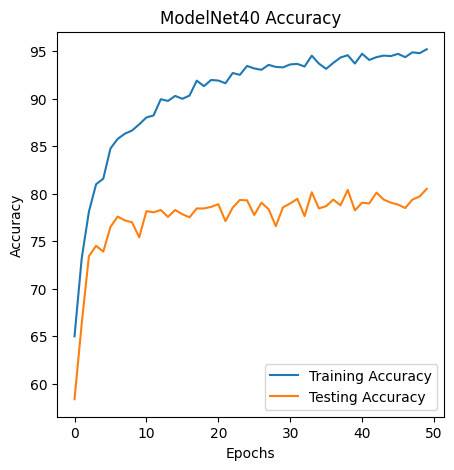
\includegraphics[scale=0.4]{Images/VoxNet/M40/acc.png}
        \includegraphics[scale=0.4]{Images/VoxNet/ShapeNet/acc.png}
        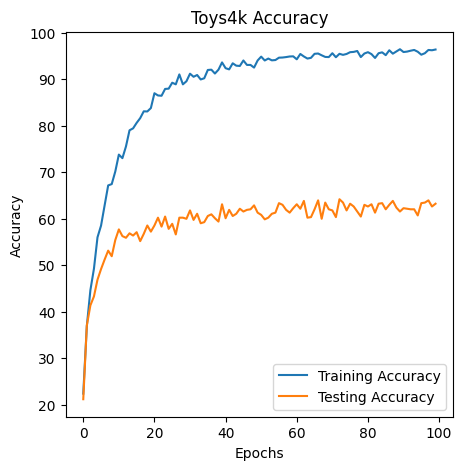
\includegraphics[scale=0.4]{Images/VoxNet/Toys4K/acc.png}
    }%
    \\
    \subfloat[Accuracy of 3DCNN Across Datasets]{%
        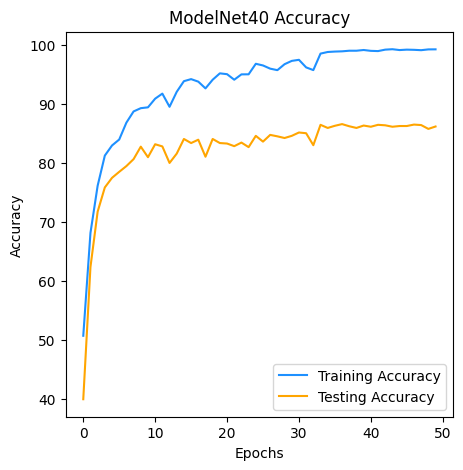
\includegraphics[scale=0.4]{Images/3DCNN/M40/acc.png}
        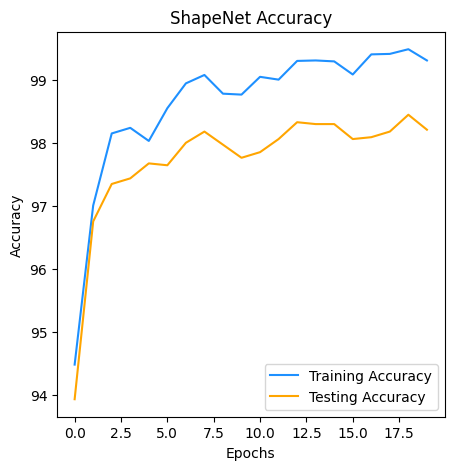
\includegraphics[scale=0.4]{Images/3DCNN/ShapeNet/acc.png}
        \includegraphics[scale=0.4]{Images/3DCNN/Toys4K/acc.png}
    }%
    \\
    \subfloat[Accuracy of Our CNN Across Datasets]{%
        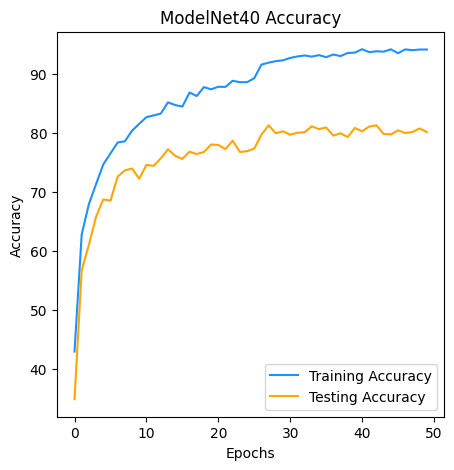
\includegraphics[scale=0.4]{Images/OurCNN/M40/acc.png}
        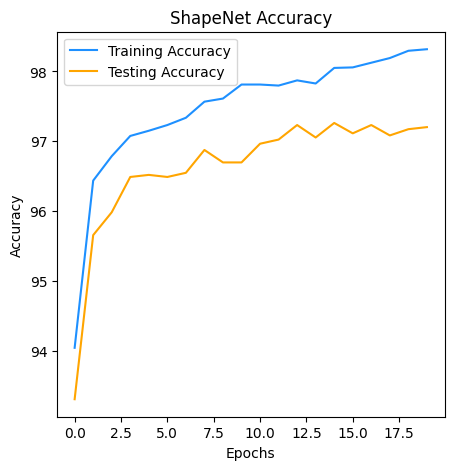
\includegraphics[scale=0.4]{Images/OurCNN/ShapeNet/acc.png}
        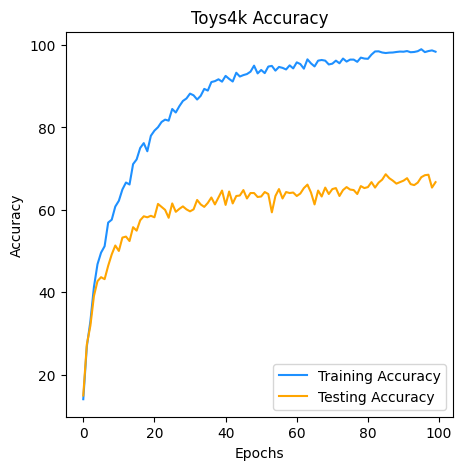
\includegraphics[scale=0.4]{Images/OurCNN/Toys4K/acc.png}
    }%
    \caption{Accuracies of CNNs across Datasets}
    \label{fig:Acc}
\end{figure*}

\begin{table}[htbp]
    \caption{Testing Accuracies of CNNs across Datasets}
    \ra{1.2}
    \begin{center}
    \begin{tabular}{|c|c|c|c|}
    \hline
    &\multicolumn{3}{|c|}{\textbf{Convolutional Neural Networks}} \\
    \cline{2-4}
    & \textbf{VoxNet} & \textbf{3DCNN} & \textbf{Our CNN} \\
    \hline
    \textbf{ModelNet40} & 80.519 & 84.984 & 80.641 \\
    \hline
    \textbf{ShapeNet} & 97.560 & 98.631 & 97.143 \\
    \hline
    \textbf{Toys4K} & 63.221 & 69.951 & 67.308 \\
    \hline
    \multicolumn{4}{l}{$^{\mathrm{a}}$Values are on average $\pm 1\%$}.
    \end{tabular}
    \label{tab1}
    \end{center}
\end{table}

\begin{table}[htbp]
    \caption{Testing F1-Scores of CNNs across Datasets}
    \ra{1.2}
    \begin{center}
    \begin{tabular}{|c|c|c|c|}
    \hline
    &\multicolumn{3}{|c|}{\textbf{Convolutional Neural Networks}} \\
    \cline{2-4}
    & \textbf{VoxNet} & \textbf{3DCNN} & \textbf{Our CNN} \\
    \hline
    \textbf{ModelNet40} & 0.806 & 0.854 & 0.808 \\
    \hline
    \textbf{ShapeNet} & 0.975 & 0.986 & 0.971 \\
    \hline
    \textbf{Toys4K} & 0.621 & 0.691 & 0.6675 \\
    \hline
    \multicolumn{4}{l}{$^{\mathrm{a}}$Values are on average $\pm 1\%$}.
    \end{tabular}
    \label{tab2}
    \end{center}
\end{table}

\begin{table}[htbp]
    \caption{Testing MSEs of CNNs across Datasets}
    \ra{1.2}
    \begin{center}
    \begin{tabular}{|c|c|c|c|}
    \hline
    &\multicolumn{3}{|c|}{\textbf{Convolutional Neural Networks}} \\
    \cline{2-4}
    & \textbf{VoxNet} & \textbf{3DCNN} & \textbf{Our CNN} \\
    \hline
    \textbf{ModelNet40} & 58.313 & 42.902 & 58.873 \\
    \hline
    \textbf{ShapeNet} & 1.43 & 0.686 & 1.77 \\
    \hline
    \textbf{Toys4K} & 628.09 & 581.310 & 550.18 \\
    \hline
    \multicolumn{4}{l}{$^{\mathrm{a}}$Values are on average $\pm 1\%$}.
    \end{tabular}
    \label{tab3}
    \end{center}
\end{table}


% --------------  DISCUSSION  -----------------

\section{Discussion}
\subsection{Findings}
In our study, we found that the overall best model was 3DCNN. This model consistently performed the best across all datasets and had the highest accuracy, F1-Score, and lowest Mean-Squared Error (except on the Toys4K dataset compared to our CNN).

Furthermore, VoxNet performed the worst out of the three models, however, it was not far behind our model. Even so, we were able to outperform the original VoxNet by a significant margin on the Toys4K dataset.

Additionally, all 3 models performed very well on the subset of ShapeNet that we used for training and testing as they all achieved accuracies and F1-Scores of over 95\% within the first few epochs. Unfortunately, the same cannot be said for the Toys4K dataset. All 3 models performed the worst on this dataset and took the longest to train.

Finally, we observed that all 3 models made the same classification mistakes when an object was misclassified. For example, all 3 models trained on ModelNet40 would misclassify desks as tables, flower pots as vases and plants, and nightstands as dressers.


\subsection{Interpretation of Findings}
\subsubsection{The Best Model}
It makes sense that 3DCNN is the best-performing model as it is the most complex of the 3 that we implemented. The trade-off for this is that it is also the most computationally expensive model out of the three. 3DCNN took the most time to train and test across all datasets. This CNN would be a good foundation for future work as it is the most accurate and has the most potential for improvement. If computing power is not an issue, this model would be the best choice for 3D object classification overall. Perhaps looking into ways to reduce the computational cost of this model without sacrificing accuracy would be a good avenue for future work. Modern 3D classification networks still follow the same basic structure as 3DCNN, with the four 3D convolutional layers. However, they have added more layers and more complex layers to improve performance.

Models like these are currently being used to perform brain tumour classification using MRI data which is commonly reconstructed into high-resolution voxelized meshes to visualize within a computer. In 2022, a method was proposed to classify brain tumours using a 3D CNN. The model used in the paper is an implementation of ResNet3D that uses 5 3D convolutional layers, a pooling layer, a dropout layer, and a fully connected layer for the output \cite{chatterjee2022}. This paper reports a consolidated macro F1-Score of 0.9095, and weighted F1-Score of 0.9269 \cite{chatterjee2022} when classifying three brain types. What is most impressive is that the mean F1-Score for the healthy brain class was 0.9998 $\pm$ 0.0002 \cite{chatterjee2022}. This is a very impressive result and should demonstrate that models like 3DCNN are a great place to start learning about 3D object classification.

\subsubsection{The Case for VoxNet}
VoxNet did perform the worst out of the three models. This was perhaps to be expected as it is the oldest of the three models and it is the least complex. However, it still outperformed our model when it came to the ShapeNet subset. All models performed very well on ShapeNet but if you are looking to classify 3D objects from a small number of classes with lots of samples, VoxNet is still not a bad choice.

Earlier in IV-B, we mentioned that our implementation of VoxNet far outperformed the original implementation. In the original research paper, VoxNet achieved an accuracy of 83.0\% on ModelNet40 using 30x30x30 voxel grids that had received data augmentation in the form of $360\degree/n$ rotations and voting. Without data augmentation, VoxNet achieved an accuracy of only 61\% when trained and tested on ModelNet40 \cite{7353481}. Our implementation of VoxNet achieved an accuracy of 80.519\% on ModelNet40 using 32x32x32 voxel grids without any data augmentation. That is a 31\% increase in accuracy over the original implementation. This indicates that as resolution increases, the performance of VoxNet increases as well. 30x30x30 voxel grids were used because they were the voxelized representations shared by the ModelNet40 research team. We find it strange that they did not produce their voxelized representations using a higher resolution because the model itself is designed to work with 32x32x32 voxel grids.

\subsubsection{Data Matters}
In the 3DCNN research paper, it is reported that they achieved an 89.34\% testing accuracy on an 18-class subset of ShapeNet with more than 45000 models\cite{gwak20153d}. They did not report which specific subset of ShapeNet they used, however, we can assume that it was very similar to the 16-class subset that we used. Using this subset, we achieved a testing accuracy of 98.631\% on CNN. Although no direct comparison can be made because of the difference in sample size, and the two extra classes, we believe that if we had access to their dataset we could achieve better results using our data preprocessing method. 

The same is true for VoxNet. Although a large portion of the ModelNet40 percent accuracy increase can be attributed to the increase in resolution, having such a large percentage increase in accuracy without data augmentation is still impressive. We believe if we were to implement a rotation transform augmentation method, we could achieve even better results using these older, easier-to-implement models.

We wish we had been able to design and evaluate a model that could take higher-resolution voxel grids as input. We believe that if we were able to do this, we could have achieved better results on all datasets. We also believe that if we were able to implement a memory partitioning strategy, we could have achieved better results on all datasets using higher-resolution voxel grids. Perhaps in the future, we will be able to implement these features and achieve better results.

\subsubsection{ShapeNet and Toys4K}
It was easily apparent that all 3 models performed the best on ShapeNet and the worst on Toys4K. This is likely because ShapeNet has the fewest classes with lots of samples, and Toys4K has the most classes with the fewest samples. It is interesting to note that our CNN performed 2.65\% worse than 3DCNN on Toys4K but managed to have a lower mean-squared error. The difference does not seem too significant but it is worth noting since this is the only dataset where our CNN performed better than 3DCNN in any metric. This could mean that given more epochs, our CNN could get closer to the performance of 3DCNN on the Toys4K dataset. The results of all models on both of these datasets demonstrate that the number of classes and samples per class in a dataset has a significant impact on the performance of a model. This also circles back to the importance of data in the field of computational intelligence.

\subsubsection{Missed Classifications}
In Fig. \ref{fig:Confusion Matrices}, we can see the confusion matrices for each model on the ModelNet40 dataset. We can see that all 3 models made the same classification mistakes when an object was misclassified. For example, all 3 models trained on ModelNet40 would misclassify desks as tables, flower pots as vases and plants, and nightstands as dressers. This is likely because these objects are very similar in shape and size. In Fig. \ref{fig:VoxNet on ModelNet40} (full images on GitHub), we can see that the model guesses that a flower pot is a plant 14 times, and a vase 8 different times. In Fig. \ref{fig:Commonly Misclassified Objects} (full images on GitHub), we can see that the flower pot and plant objects are very similar, and this is just one such example.

Furthermore, another interesting thing to note is that in Fig. \ref{fig:3DCNN on ModelNet40} we can see that the model is better at classifying everything except for two classes. It consistently thinks that a desk is a table, and a flower pot is a plant. This proves that even though 3DCNN is the most accurate, it is not perfect. It is important to note that if these models were to be used in a real-world application, they would need to be trained on a much larger dataset with more classes and samples per class. In the case of similar flower pot and plant models, we think it would be best to put the objects from the plant class into the flower pot class if it is indeed a potted plant. This would most likely result in higher accuracy for the model as there is no way for the model to tell the difference between a potted plant labeled as a plant and a potted plant labeled as a flower pot.

\begin{figure*}
    \centering
    \subfloat[VoxNet on ModelNet40]{%
        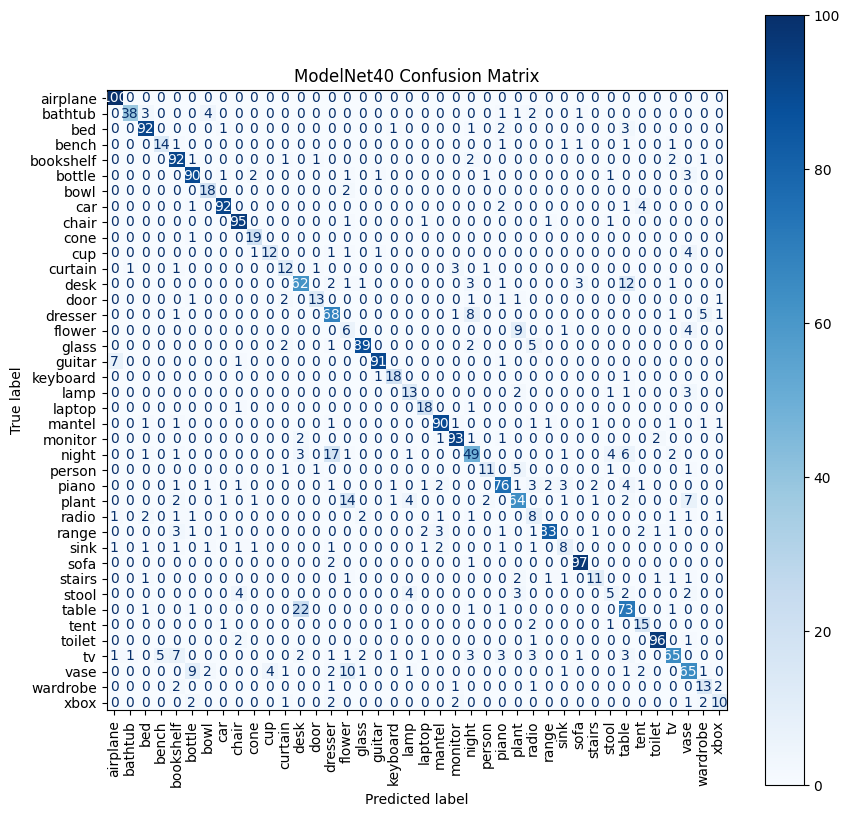
\includegraphics[scale=0.28]{Images/VoxNet/M40/cm.png}
        \label{fig:VoxNet on ModelNet40}
    }%
    \subfloat[3DCNN on ModelNet40]{%
        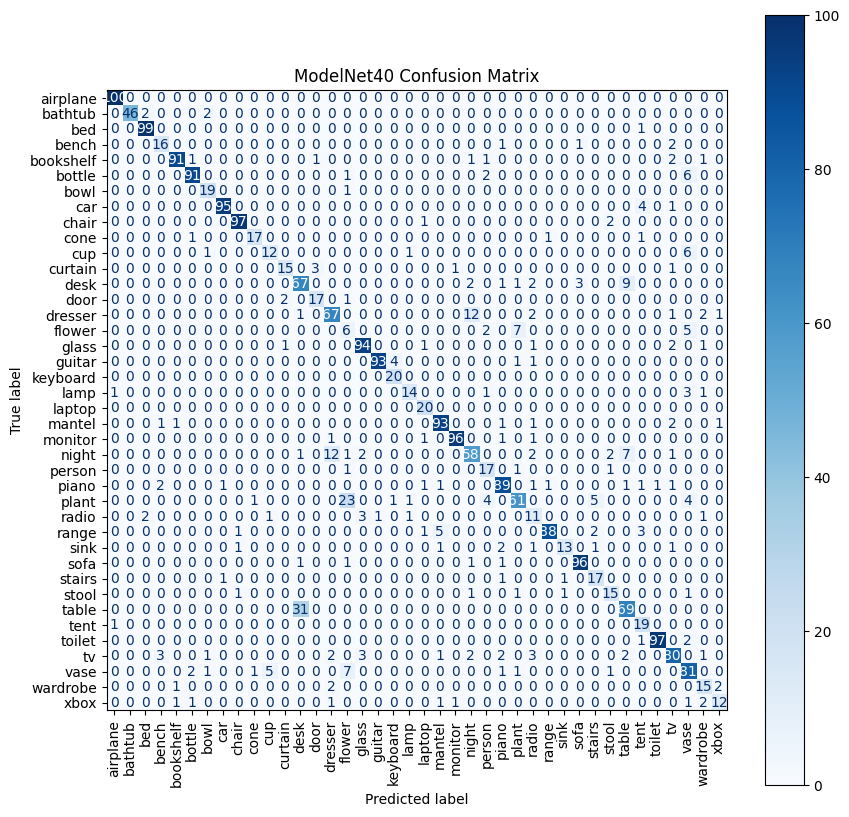
\includegraphics[scale=0.28]{Images/3DCNN/M40/cm.png}
        \label{fig:3DCNN on ModelNet40}
    }%
    \subfloat[Our CNN on ModelNet40]{
        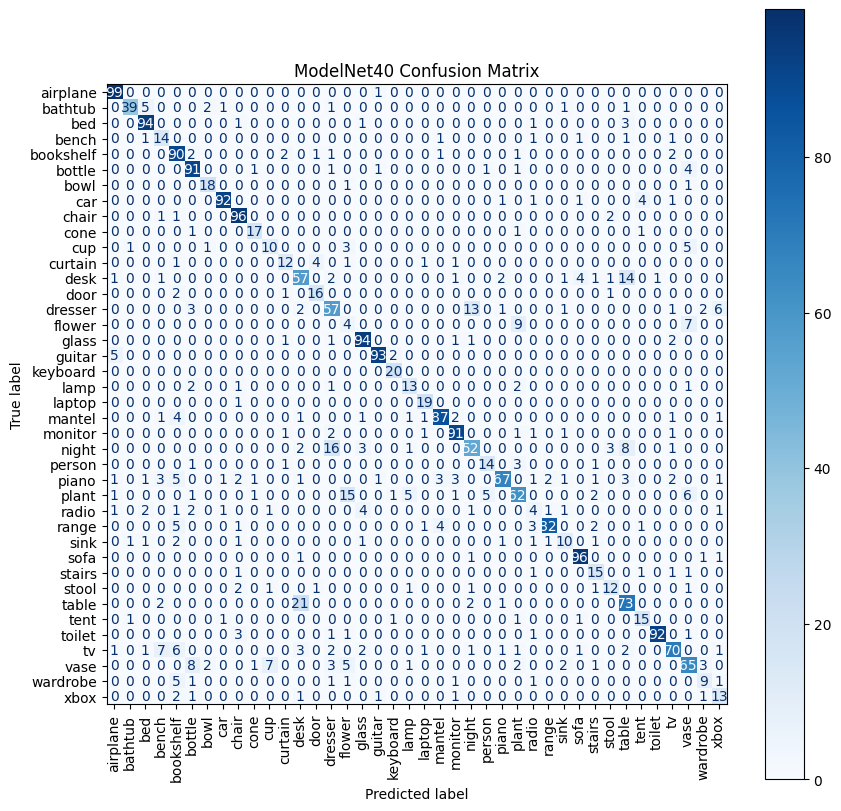
\includegraphics[scale=0.28]{Images/OurCNN/M40/cm.png}
        \label{fig:Our CNN on ModelNet40}
    }%
    \caption{Confusion Matrices of CNNs on ModelNet40}
    \label{fig:Confusion Matrices}
\end{figure*}

\begin{figure*}
    \centering
    \subfloat[Voxelized Flower Pot Sample]{%
        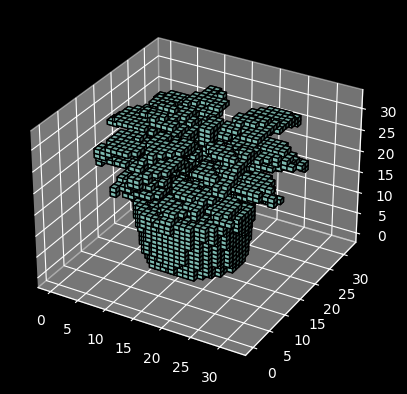
\includegraphics[scale=0.5]{Images/flower pot.png}
        \label{fig:Flower Pot}
    }%
    \subfloat[Voxelized Plant Sample]{
        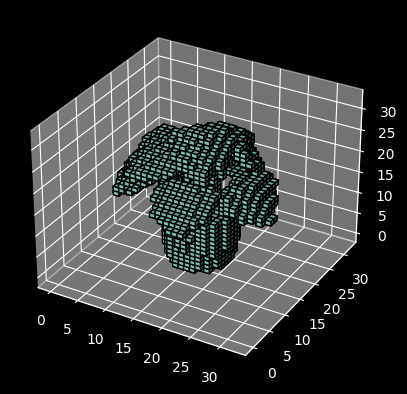
\includegraphics[scale=0.5]{Images/plant.png}
        \label{fig:Vase}
    }%
    \caption{Commonly Misclassified Objects}
    \label{fig:Commonly Misclassified Objects}
\end{figure*}

\subsection{Pros and Cons}

\subsubsection{VoxNet}
\begin{list}{\labelitemi}{\leftmargin=1em}
    \item Pros
    \begin{list}{\labelitemii}{\leftmargin=1em}
        \item Simple to implement.
        \item Fast to train and test.
        \item Performs well on datasets with few classes and lots of samples.
    \end{list}
    \item Cons
    \begin{list}{\labelitemii}{\leftmargin=1em}
        \item Performs poorly on datasets with lots of classes and few samples.
        \item Can perform poorly on datasets that have not been augmented \cite{7353481}.
    \end{list}
\end{list}
\
\subsubsection{3DCNN}
\begin{list}{\labelitemi}{\leftmargin=1em}
    \item Pros
    \begin{list}{\labelitemii}{\leftmargin=1em}
        \item Performs the best out of the 3 models.
        \item Performs best on datasets with lots of classes and few samples.
        \item Performs best on datasets with few classes and lots of samples.
        \item Performs best overall.
    \end{list}
    \item Cons
    \begin{list}{\labelitemii}{\leftmargin=1em}
        \item Very slow to train and test compared to the other models.
        \item Complex to implement.
    \end{list}
\end{list}
\
\subsubsection{Our CNN}
\begin{list}{\labelitemi}{\leftmargin=1em}
    \item Pros
    \begin{list}{\labelitemii}{\leftmargin=1em}
        \item Performs well on datasets with lots of classes and few samples.
        \item Performs well on datasets with few classes and lots of samples.
        \item Performs well on datasets that have not been augmented.
        \item Fast to train and test.
        \item Simple to implement.
    \end{list}
    \item Cons
    \begin{list}{\labelitemii}{\leftmargin=1em}
        \item Performs the worst on datasets with few classes and lots of samples.
        \item Could use some changes to the architecture to improve performance.
    \end{list}
\end{list}
% --------------  CONCLUSION  -----------------

\section{Conclusion}
Overall, we can see that each model performs similarly to the others when we compare their accuracy, F-1 score, mean-squared error, and confusion grids. Notably, our CNN offers better results than VoxNet on more diverse datasets, while being a less computationally expensive model relative to 3DCNN. This illustrates our belief that the capabilities of machine learning would be readily apparent through the comparison of the algorithms of then versus now. This is to be expected, as our CNN was based on the works of both papers, as well as what we learned throughout the semester. Furthermore, when comparing the models' accuracies to their reported accuracies in the papers that first created them, we showed a significant increase in their performance even compared to previous versions of the same models. We believe that this also highlights the benefits of our simple voxelization process since our results match those of the other models trained on augmented datasets. This further demonstrates the clear evolution of computational intelligence over the years, and that the data that is given to models is just as important, if not more important, than the models themselves. In the future, we believe it would be wise to further research these models using our data framework with data augmentation techniques such as rotation transformations.

In conclusion, we believe that our findings offer valuable insights into the capabilities of older 3D classification CNNs, and their ability to still perform well even in the modern day.

% For papers published in translation journals, please give the English 
% citation first, followed by the original foreign-language citation \cite{b6}.

% Citations of a reference should be done using the \cite{} command. 
% Once cited, they will appear in the references section at the end of the document. 
%The \cite{} command can also take in a page number as an argument, for example \cite[page 5]{}.
\bibliographystyle{IEEEtran}
\bibliography{bibliography}

\end{document}